% Standalone source of the four sectors of the three-vertex chain
% (Sec. 5, first example), drawn in the same visual language as the original
% three_vertex_tree figure and as figure fig_tree_diagram: hatched-circle
% components, open-square leg tips and teal propagator labels above the
% surviving line. A contracted propagator is absent and its vertices merge into
% one larger hatched circle; the merged component carries a single regular,
% evenly spaced external-leg fan labelled by the SUM of the merged vertices'
% external energies (E_1+E_2 etc.), while an unmerged vertex keeps its own
% two-leg fan and its own energy label.
% Compile: pdflatex fig_tree_sectors.tex   (included by paper.tex)
\documentclass[tikz,border=6pt]{standalone}
\usetikzlibrary{patterns.meta,calc}
\definecolor{propteal}{RGB}{0,166,172}
\tikzset{
  vtx/.style={circle, draw=black, line width=1.0pt, fill=white,
    postaction={pattern={Lines[angle=45, distance=1.3pt, line width=0.45pt]},
      pattern color=black},
    minimum size=#1, inner sep=0pt, outer sep=0pt},
  vtx/.default=4.2pt,
  leg/.style={draw=black, line width=0.9pt},
  sq/.style={draw=black, line width=0.9pt, fill=white, minimum size=3.0pt,
    inner sep=0pt, outer sep=0pt},
  prop/.style={line width=1.2pt},
}
% Two-leg fan of an unmerged end vertex, energy label beside the fan.
\newcommand{\fanL}[2]{%
  \draw[leg] (#1) -- ++(149:1.52) node[sq] {};
  \draw[leg] (#1) -- ++(200:1.45) node[sq] {};
  \node at ($(#1)+(-1.02,1.06)$) {\footnotesize $#2$};
}
\newcommand{\fanM}[2]{%
  \draw[leg] (#1) -- ++(120:1.85) node[sq] {};
  \draw[leg] (#1) -- ++(60:1.85)  node[sq] {};
  \node at ($(#1)+(0,2.10)$) {\footnotesize $#2$};
}
\newcommand{\fanR}[2]{%
  \draw[leg] (#1) -- ++(31:1.52)  node[sq] {};
  \draw[leg] (#1) -- ++(-20:1.45) node[sq] {};
  \node at ($(#1)+(1.02,1.06)$) {\footnotesize $#2$};
}
% Regular evenly spaced upward fan of a merged component, labelled by the
% summed external energy of all merged vertices.
\newcommand{\fanSymFour}[2]{%
  \foreach \a in {150,110,70,30} { \draw[leg] (#1) -- ++(\a:1.7) node[sq] {}; }
  \node at ($(#1)+(0,2.15)$) {\footnotesize $#2$};
}
\newcommand{\fanSymSix}[2]{%
  \foreach \a in {150,126,102,78,54,30} { \draw[leg] (#1) -- ++(\a:1.7) node[sq] {}; }
  \node at ($(#1)+(0,2.15)$) {\footnotesize $#2$};
}
\begin{document}
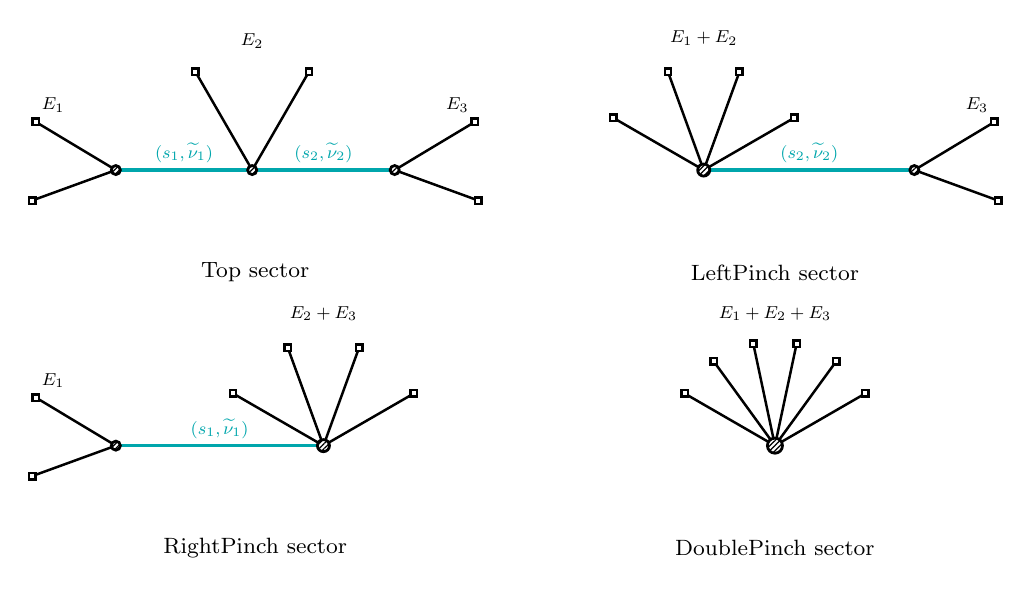
\begin{tikzpicture}[every node/.style={inner sep=1.5pt}]
  % Top sector: the full chain, three unmerged vertices.
  \begin{scope}[shift={(0,0)}, scale=0.78, transform shape]
    \coordinate (tL) at (0,0);
    \coordinate (tM) at (2.22,0);
    \coordinate (tR) at (4.54,0);
    \fanL{tL}{E_1}\fanM{tM}{E_2}\fanR{tR}{E_3}
    \draw[prop,propteal] (tL) -- (tM);
    \draw[prop,propteal] (tM) -- (tR);
    \node[propteal] at (1.11,0.28) {\footnotesize $(s_1,\widetilde\nu_1)$};
    \node[propteal] at (3.38,0.28) {\footnotesize $(s_2,\widetilde\nu_2)$};
    \node[vtx] at (tL) {}; \node[vtx] at (tM) {}; \node[vtx] at (tR) {};
  \end{scope}
  \node at (1.77,-1.30) {\footnotesize Top sector};
  % LeftPinch: propagator 1 contracted, L and M merged.
  \begin{scope}[shift={(6.6,0)}, scale=0.78, transform shape]
    \coordinate (mLM) at (1.11,0);
    \coordinate (pR)  at (4.54,0);
    \fanSymFour{mLM}{E_1+E_2}
    \fanR{pR}{E_3}
    \draw[prop,propteal] (mLM) -- (pR);
    \node[propteal] at (2.83,0.28) {\footnotesize $(s_2,\widetilde\nu_2)$};
    \node[vtx=5.6pt] at (mLM) {}; \node[vtx] at (pR) {};
  \end{scope}
  \node at (8.37,-1.30) {\footnotesize LeftPinch sector};
  % RightPinch: propagator 2 contracted, M and R merged.
  \begin{scope}[shift={(0,-3.5)}, scale=0.78, transform shape]
    \coordinate (qL)  at (0,0);
    \coordinate (mMR) at (3.38,0);
    \fanL{qL}{E_1}
    \fanSymFour{mMR}{E_2+E_3}
    \draw[prop,propteal] (qL) -- (mMR);
    \node[propteal] at (1.69,0.28) {\footnotesize $(s_1,\widetilde\nu_1)$};
    \node[vtx] at (qL) {}; \node[vtx=5.6pt] at (mMR) {};
  \end{scope}
  \node at (1.77,-4.80) {\footnotesize RightPinch sector};
  % DoublePinch: both propagators contracted, all vertices merged.
  \begin{scope}[shift={(6.6,-3.5)}, scale=0.78, transform shape]
    \coordinate (mD) at (2.27,0);
    \fanSymSix{mD}{E_1+E_2+E_3}
    \node[vtx=7.0pt] at (mD) {};
  \end{scope}
  \node at (8.37,-4.80) {\footnotesize DoublePinch sector};
\end{tikzpicture}
\end{document}
